% Author: Alfredo Fánchez Alberca (asalber@ceu.es)

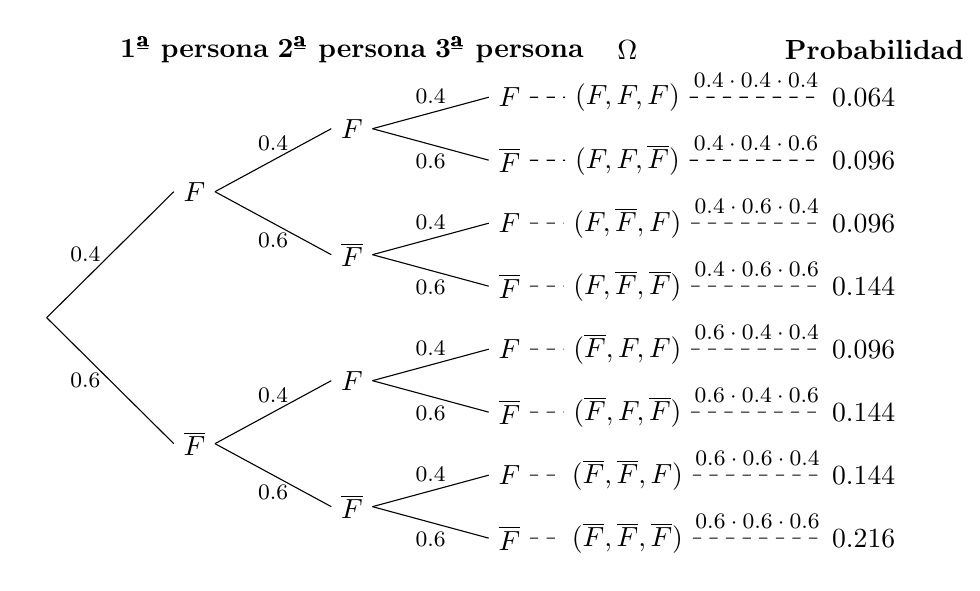
\begin{tikzpicture}[
grow'=right,
% sloped,
level 1/.style ={level distance=2cm, sibling distance=3.2cm, parent anchor=east, child anchor=west},
level 2/.style ={level distance=2cm, sibling distance=1.6cm},
level 3/.style ={level distance=2cm, sibling distance=0.8cm},
level 4/.style ={level distance=1.5cm, sibling distance=0.8cm, dashed},
level 5/.style ={level distance=3cm, sibling distance=0.8cm, dashed},
prob/.style={font=\footnotesize,above}
]

\node (root) {}
	child {node {$F$}
		child {node {$F$}
	   		child {node {$F$}
				child {node{$(F,F,F)$}
					child {node {$0.064$} edge from parent node[prob] {$0.4\cdot 0.4\cdot 0.4$}} 
				}
				edge from parent node[prob] {$0.4$}
			}
			child {node {$\overline F$}
				child {node{$(F,F,\overline F)$}
					child {node {$0.096$} edge from parent node[prob] {$0.4\cdot 0.4\cdot 0.6$}}
				}
				edge from parent node[prob,below] {$0.6$}
			}
			edge from parent node[prob] {$0.4$}
		}
		child {node {$\overline F$}
	   		child {node {$F$}
				child {node{$(F,\overline F,F)$}
					child {node{$0.096$} edge from parent node[prob] {$0.4\cdot 0.6\cdot 0.4$}}
				}
				edge from parent node[prob] {$0.4$}
			}
			child {node {$\overline F$}
				child {node{$(F,\overline F,\overline F)$}
					child {node{$0.144$} edge from parent node[prob] {$0.4\cdot 0.6\cdot 0.6$}}
				}
				edge from parent node[prob,below] {$0.6$}
			}
			edge from parent node[prob,below] {$0.6$}
		}
		edge from parent node[prob,left] {$0.4$}
	}
	child {node {$\overline F$}
		child {node {$F$}
	   		child {node {$F$}
				child {node{$(\overline F,F,F)$}
					child {node {$0.096$} edge from parent node[prob] {$0.6\cdot 0.4\cdot 0.4$}} 
				}
				edge from parent node[prob] {$0.4$}
			}
			child {node {$\overline F$}
				child {node{$(\overline F,F,\overline F)$}
					child {node {$0.144$} edge from parent node[prob] {$0.6\cdot 0.4\cdot 0.6$}}
				}
				edge from parent node[prob,below] {$0.6$}
			}
			edge from parent node[prob] {$0.4$}
		}
		child {node {$\overline F$}
	   		child {node {$F$}
				child {node{$(\overline F,\overline F,F)$}
					child {node{$0.144$} edge from parent node[prob] {$0.6\cdot 0.6\cdot 0.4$}}
				}
				edge from parent node[prob] {$0.4$}
			}
			child {node {$\overline F$}
				child {node{$(\overline F,\overline F,\overline F)$}
					child {node{$0.216$} edge from parent node[prob] {$0.6\cdot 0.6\cdot 0.6$}}
				}
				edge from parent node[prob,below] {$0.6$}
			}
			edge from parent node[prob,below] {$0.6$}
		}
		edge from parent node[prob,left] {$0.6$}
	};

\begin{scope}[every node/.style={text width=2cm, align=center, anchor=center, font=\bfseries,}]
\node (labels-level) at ([yshift=0.6cm]root-1-1-1-1-1) {Probabilidad};
\node[at =(labels-level-|root-1)] {1ª persona};
\node[at =(labels-level-|root-1-1)] {2ª persona};
\node[at =(labels-level-|root-1-1-1)] {3ª persona};
\node[at =(labels-level-|root-1-1-1-1)]{$\Omega$};
\end{scope}
\end{tikzpicture}
